\documentclass{article}

\usepackage{amsmath,amssymb}
\usepackage{tikz}
\usepackage{pgfplots}
\usepackage{xcolor}
\usepackage[left=2.1cm,right=3.1cm,bottom=3cm,footskip=0.75cm,headsep=0.5cm]{geometry}
\usepackage{enumerate}
\usepackage{enumitem}
\usepackage{marvosym}
\usepackage{tabularx}
\usepackage{parskip}
\usepackage{multirow}
\usepackage{dcolumn}
\usepackage{longtable}
\usepackage[backend=bibtex]{biblatex}
\addbibresource{refs}
\bibliography{refs}

\usepackage{listings}
\definecolor{lightlightgray}{rgb}{0.95,0.95,0.95}
\definecolor{lila}{rgb}{0.8,0,0.8}
\definecolor{mygray}{rgb}{0.5,0.5,0.5}
\definecolor{mygreen}{rgb}{0,0.8,0.26}
%\lstdefinestyle{java} {language=java}
\lstset{language=R,
	basicstyle=\ttfamily,
	keywordstyle=\color{lila},
	commentstyle=\color{lightgray},
	stringstyle=\color{mygreen}\ttfamily,
	backgroundcolor=\color{white},
	showstringspaces=false,
	numbers=left,
	numbersep=10pt,
	numberstyle=\color{mygray}\ttfamily,
	identifierstyle=\color{blue},
	xleftmargin=.1\textwidth, 
	%xrightmargin=.1\textwidth,
	escapechar=§,
	%literate={\t}{{\ }}1
	breaklines=true,
	postbreak=\mbox{\space},
	morekeywords={test}
}

\usepackage[colorlinks = true, linkcolor = blue, urlcolor  = blue, citecolor = blue, anchorcolor = blue]{hyperref}
\usepackage[utf8]{inputenc}

\renewcommand*{\arraystretch}{1.4}

\newcolumntype{L}[1]{>{\raggedright\arraybackslash}p{#1}}
\newcolumntype{R}[1]{>{\raggedleft\arraybackslash}p{#1}}
\newcolumntype{C}[1]{>{\centering\let\newline\\\arraybackslash\hspace{0pt}}m{#1}}

\newcommand{\E}{\mathbb{E}}
\DeclareMathOperator{\rk}{rk}
\DeclareMathOperator{\Var}{Var}
\DeclareMathOperator{\Cov}{Cov}

\title{\textbf{Econometrics 2, Assignment 1}}
\author{\textsc{Henry Haustein}}
\date{}

\begin{document}
	\maketitle
	
	\section*{Section A: Proof of Variance}
	\begin{enumerate}[label=(\alph*)]
		\item We start by showing $\sum (W_i-\bar{W})^2 = N\bar{W}(1-\bar{W}) = \left(\frac{1}{N_c} + \frac{1}{N_t}\right)^{-1}$:
		\begin{align}
			\sum_{i=1}^N (W_i-\bar{W})^2 &= \sum_{i=1}^N W_i^2 - 2\bar{W}\underbrace{\sum_{i=1}^N W_i}_{N\bar{W}} + N\bar{W}^2 \notag \\
			&= \sum_{i=1}^N W_i^2 - N\bar{W}^2 \notag \\
			&= N\bar{W} - N\bar{W}^2 \label{eq:1} \\
			&= N\bar{W}(1-\bar{W}) \notag \\
			&= N\frac{N_t}{N}\cdot\frac{N_c}{N} \notag \\
			&= \frac{N_tN_c}{N} \label{eq:2} \\
			&= \frac{N_tN_c}{N_t+N_c} \notag \\
			&= \left(\frac{1}{N_c} + \frac{1}{N_t}\right)^{-1} \notag
		\end{align}
		where we use in \eqref{eq:1} the fact that for $W\in\{0,1\}$ $W = W^2$.
		
		We can now show that $V^{const} = V^{homo}$:
		\begin{align}
			V^{const} &= s^2\left(\frac{1}{N_c} + \frac{1}{N_t}\right) \notag \\
			&= \frac{1}{N-2}\left((N_c-1)\frac{1}{N_c-1}\sum_{W_i:i=0}(Y_i-\bar{Y}_c)^2 + (N_t-1)\frac{1}{N_t-1}\sum_{W_i:i=1}(Y_i-\bar{Y}_t)^2\right)\left(\frac{1}{N_c} + \frac{1}{N_t}\right) \notag \\
			&= \frac{1}{N-2}\left(\sum_{W_i:i=0}(Y_i-\bar{Y}_c)^2 + \sum_{W_i:i=1}(Y_i-\bar{Y}_t)^2\right)\left(\frac{1}{N_c} + \frac{1}{N_t}\right) \notag \\
			&= \frac{1}{N-2}\left(\sum_{W_i:i=0}(Y_i-\bar{Y}_c)^2 + \sum_{W_i:i=1}(Y_i-\bar{Y}_t)^2\right)\left(\frac{1}{N_c} + \frac{1}{N_t}\right) \cdot \frac{\left(\frac{1}{N_c} + \frac{1}{N_t}\right)^{-1}}{\left(\frac{1}{N_c} + \frac{1}{N_t}\right)^{-1}} \notag \\
			&= \frac{\frac{1}{N-2}\left(\sum_{W_i:i=0}(Y_i-\bar{Y}_c)^2 + \sum_{W_i:i=1}(Y_i-\bar{Y}_t)^2\right)}{\left(\frac{1}{N_c} + \frac{1}{N_t}\right)^{-1}} \notag \\
			&= \frac{\frac{1}{N-2}\left(\sum_{W_i:i=0}(Y_i-\bar{Y}_c)^2 + \sum_{W_i:i=1}(Y_i-\bar{Y}_t)^2\right)}{\sum_{i=1}^N (W_i-\bar{W})^2} \notag \\
			&= \frac{\hat{\sigma^2_\varepsilon}}{\sum_{i=1}^N (W_i-\bar{W})^2} \notag \\
			&= V^{homo} \notag
		\end{align}
		\item We show $V^{hetero} = V^{neyman}$:
		\begin{align}
			V^{hetero} &= \frac{\sum_{i=1}^N \hat{\varepsilon}_i^2\cdot (W_i-\bar{W})^2}{\left(\sum_{i=1}^N (W_i-\bar{W})^2\right)^2} \notag \\
			&= \frac{\sum_{i=1}^N (Y_i-\alpha^{OLS} - \beta^{OLS}W_i)^2\cdot (W_i-\bar{W})^2}{\left(\sum_{i=1}^N (W_i-\bar{W})^2\right)^2} \notag \\
			&= \frac{\sum_{i=1}^N (Y_i-\bar{Y}-(\bar{Y}_t - \bar{Y}_c)(W_i-\bar{W}))^2\cdot (W_i-\bar{W})^2}{\left(\sum_{i=1}^N (W_i-\bar{W})^2\right)^2} \notag \\
			\intertext{We are now using the fact that $\bar{Y} = \bar{W}\bar{Y}_t + (1-\bar{W})\bar{Y}_c$}
			&= \frac{\sum_{W_i:i=0} (Y_i-\bar{W}\bar{Y}_t - (1-\bar{W})\bar{Y}_c + \bar{Y}_t\bar{W} - \bar{Y}_c\bar{W})^2\cdot (-\bar{W})^2}{\left(\sum_{i=1}^N (W_i-\bar{W})^2\right)^2} \notag \\
			&+ \frac{\sum_{W_i:i=1} (Y_i-\bar{W}\bar{Y}_t - (1-\bar{W})\bar{Y}_c - \bar{Y}_t + \bar{Y}_t\bar{W} + \bar{Y}_c - \bar{Y}_c\bar{W})^2\cdot (1-\bar{W})^2}{\left(\sum_{i=1}^N (W_i-\bar{W})^2\right)^2} \notag \\
			&= \frac{\sum_{W_i:i=0} (Y_i-\bar{Y}_c)^2\cdot (-\bar{W})^2 + \sum_{W_i:i=1} (Y_i-\bar{Y}_t)^2\cdot(1-\bar{W})^2}{\left(\sum_{i=1}^N (W_i-\bar{W})^2\right)^2} \notag \\
			&= \frac{\left(\frac{N_t}{N}\right)^2\sum_{W_i:i=0} (Y_i-\bar{Y}_c)^2 + \left(\frac{N_c}{N}\right)^2\sum_{W_i:i=1} (Y_i-\bar{Y}_t)^2}{\left(\sum_{i=1}^N (W_i-\bar{W})^2\right)^2} \notag \\
			\intertext{using \eqref{eq:2}}
			&= \frac{\frac{N_t^2}{N^2}\sum_{W_i:i=0} (Y_i-\bar{Y}_c)^2 + \frac{N_c^2}{N^2}\sum_{W_i:i=1} (Y_i-\bar{Y}_t)^2}{\left(\frac{N_tN_c}{N}\right)^2} \notag \\
			&= \frac{1}{N_c^2}\sum_{W_i:i=0} (Y_i-\bar{Y}_c)^2 + \frac{1}{N_t^2}\sum_{W_i:i=1}(Y_i-\bar{Y}_t)^2 \notag \\
			&= \frac{\tilde{s}_c^2}{N_c} + \frac{\tilde{s}_t^2}{N_t} \notag \\
			&= V^{neyman} \notag
		\end{align}
		\item Homogeneous treatment effects mean that the treatment effect is the same for every individual. Then the variance of the outcome $Y$ is only coming from the error term $\varepsilon_i$ (and this variance is the same for every one). This means we have homoscedasticity.
	\end{enumerate}

	\section*{Section B: Power Calculation}
	We can calculate the power of a $t$-test pretty fast with R's \texttt{power.t.test} function (we have to set $n=400$ because the $n$ we pass to the \texttt{power.t.test} function is the $n$ for each group: sample size of 800 and 2 groups $\Rightarrow n = 400$):
	\begin{lstlisting}
power.t.test(n = 400, delta = 0.207)
	\end{lstlisting}
	returns a power of 0.8324603. But there's a problem: We don't split our sample size in 2 \textit{equal} groups. One group has 480 dyads (60\% of 800), the other one has 320 dyads (40\% of 800). We could make our life easy and do a linear approximation of the power function between $n=320$ and $n=480$:
	\begin{lstlisting}
power.t.test(n = c(320,480), delta = 0.207)
	\end{lstlisting}
	gives a power of \texttt{c(0.7435918, 0.8931858)} so on average a power of: $\frac{0.7435918 + 0.8931858}{2} = 0.8183888$. 
	
	How are these numbers calculated? As the power of a test is the probability of rejecting $H_0$ when $H_1$ is true, we draw our sample from a $t$ distribution with $2(n-1)$ degrees of freedom and a non-centrality-parameter of $\sqrt{\frac{n}{2}}\cdot\frac{\delta}{\sigma}$. We are interested that our realisation will fall in the rejection region of $H_0$ which is outside of $[t_{df,\alpha/2},t_{df,1-\alpha/2}]$\footnote{As I learned stats in Germany I'm following the German notation which might be different that the notation taught here. With $t_{df,\alpha/2}$ I mean the $\alpha/2$ quantile of the $t$-distribution with $df$ degrees of freedom.}. The critical values are
	\begin{lstlisting}
qt(0.025, 798)
qt(0.975, 798)
	\end{lstlisting}
	which are -1.962941 and 1.962941. Then the probability of being outside of $[t_{df,\alpha/2},t_{df,1-\alpha/2}]$ (when $H_1$ is true) is
	\begin{align}
		\mathbb{P}(X\notin [t_{df,\alpha/2},t_{df,1-\alpha/2}]) &= 1 - \mathbb{P}(X\in [t_{df,\alpha/2},t_{df,1-\alpha/2}]) \notag \\
		&= 1 - [\mathbb{P}(X\le ,t_{df,1-\alpha/2}) - \mathbb{P}(X \le t_{df,\alpha/2})] \notag
	\end{align}
	where $X\sim \mathcal{T}(df, ncp)$ and $ncp = \sqrt{\frac{n}{2}}\cdot\frac{\delta}{\sigma} = \sqrt{\frac{400}{2}}\cdot\frac{0.207\sigma}{\sigma} = 2.927422$
	\begin{lstlisting}
ncp = sqrt(200)*0.207
1 - (pt(1.962941, df = 798, ncp = ncp) - pt(-1.962941, df = 798, ncp = ncp))
	\end{lstlisting}
	returns 0.8324609.
	
	But we can get more accurate: Following \cite{Dalgaard2008} the non-centrality-parameter for groups with an unequal size is
	\begin{align}
		ncp &= \frac{\delta}{\sigma\sqrt{\frac{1}{n_1} + \frac{1}{n_2}}} \notag \\
		&= \frac{0.207\sigma}{\sigma\sqrt{\frac{1}{320} + \frac{1}{480}}} \notag \\
		&= 2.868276 \notag
	\end{align}
	This leads then to
	\begin{lstlisting}
ncp = 0.207/sqrt(1/320 + 1/480)
1 - (pt(1.962941, df = 798, ncp = ncp) - pt(-1.962941, df = 798, ncp = ncp))
\end{lstlisting}	
	which is 0.8172306.

	\section*{Section C: Simulation Exercise}
	The 5 model specifications are:
	\begin{lstlisting}[tabsize=2]
# Model 1
m1 = lm(Y ~ W)

# Model 2
m2 = lm(Y ~ W + age + female + age*female) # this is the same as m2 = lm(Y ~ W + age*female)

# Model 3
agematrix = matrix(0, nrow = observations, ncol = 65-20+1)
for (i in 1:observations) {
	currentAge = age[i]
	agematrix[i, currentAge - 20 + 1] = 1
}
m3 = lm(Y ~ W + agematrix + 0) # could have achieved the same with declaring age as a factor

# Model 4
logitModel = glm(W ~ age, family = binomial(logit))
propScore = predict.glm(logitModel, newdata = as.list(age), type = "response")
lambda = 1/(propScore^W * (1 - propScore)^(1-W))
m4 = lm(Y ~ W, weights = lambda)

# Model 5
logitModel2 = glm(W ~ agematrix + 0, family = binomial(logit))
propScore2 = predict.glm(logitModel2, newdata = as.list(age), type = "response")
lambda2 = 1/(propScore2^W * (1 - propScore2)^(1-W))
m5 = lm(Y ~ W, weights = lambda2)
	\end{lstlisting}
	You can see the whole R code in the attached file. The kernel-density plot is
	\begin{center}
		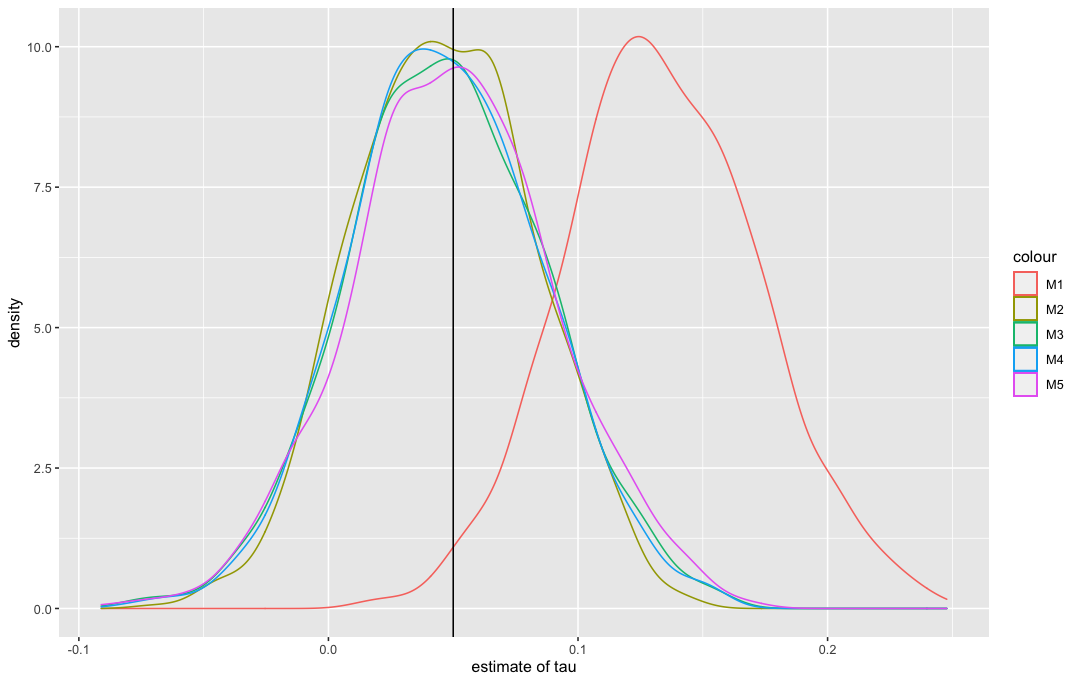
\includegraphics[scale=0.3]{kde}
	\end{center}
	where we can see:
	\begin{itemize}
		\item Model 1 has a omitted variable bias since we didn't include \texttt{female} and \texttt{age}. We can check from what variable the OVB comes with \texttt{cor.test()}:
		\begin{lstlisting}
cor.test(W, female)
cor.test(W, age)
		\end{lstlisting}
		The first test results in a p-value of 0.2356; the second test has a p-value of $2.314\cdot 10^{-8}$. This means in the first test we can't reject the Null hypothesis but we reject it in the second test. So there is a significant correlation between \texttt{W} and \texttt{age} but not between \texttt{W} and \texttt{female}. The OVB comes from \texttt{age}.
		\item Model 2 is the same specification then the data generation process so we except no OVB and see that there is no OVB.
		\item Model 3 doesn't show any OVB either but this is not a surprise after we've seen in the analysis of model 1 that \texttt{female} has no significant correlation with \texttt{W}. So removing \texttt{female} from the model and using a saturated model with \texttt{age} can capture all the variance from \texttt{female} (which comes from \texttt{age} by construction) and we see the same KDE for $\hat{\tau}$ as model 2.
		\item Model 4 has the same specification than model 1 so we would expect a OVB on \texttt{age}. But in the plot we don't see a OVB. According to \cite{Hernan2004} page 620 the method of using inverse probability weights adjusts for selection bias.
		\item The same is valid for model 5.
	\end{itemize}

	\section*{Section D: Differences-in-differences}
	Before going to the tasks let's have a look on the missing data:
	\begin{lstlisting}
library(haven)
library(naniar)
library(ggplot2)

data = read_dta("lfs_2010_2019_ages1564_20per.dta")
gg_miss_var(data) + labs(y = "Look at all the missing ones")
	\end{lstlisting}
	We get the following plot:
	\begin{center}
		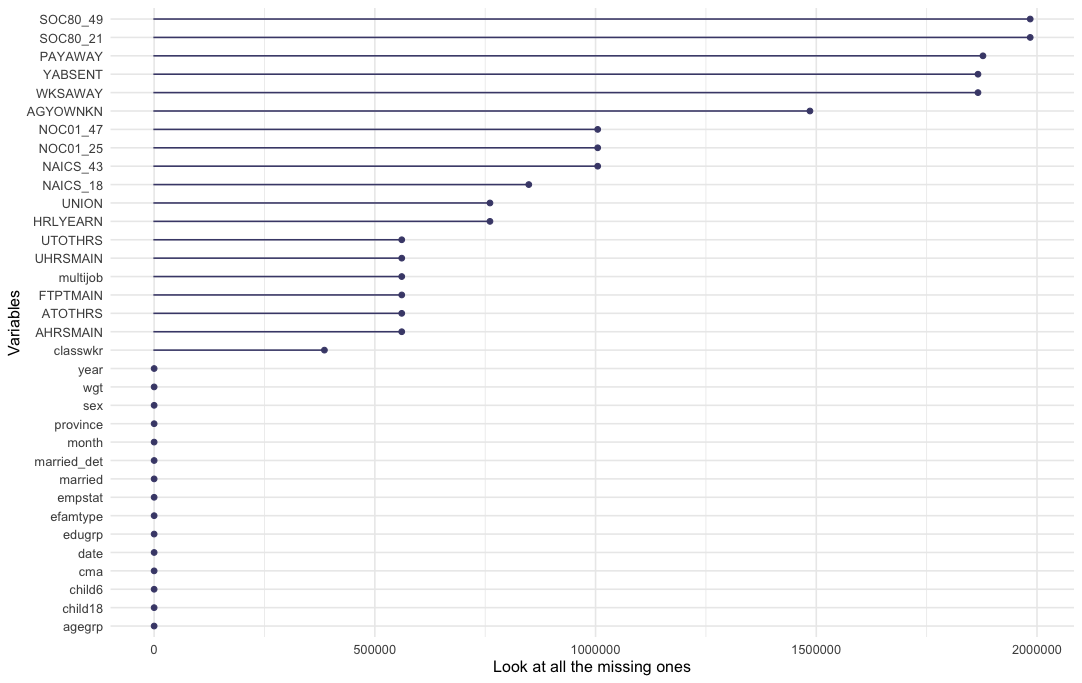
\includegraphics[scale = 0.4]{missing_values}
	\end{center}
	I don't want to deal with missing data and luckily I don't need to when fitting the models in (c).
	\begin{enumerate}[label=(\alph*)]
		\item From the lecture notes \textit{Like controlled experiments, natural experiments create the conditions of a treated and control group. BUT without random assignment, these groups are not directly comparably.} The policy change divides the population of Canada into a treatment and control group but there might be spillover effect since people can move from one state to another state.
		\item The plot for the yearly employment rate is
		\begin{center}
			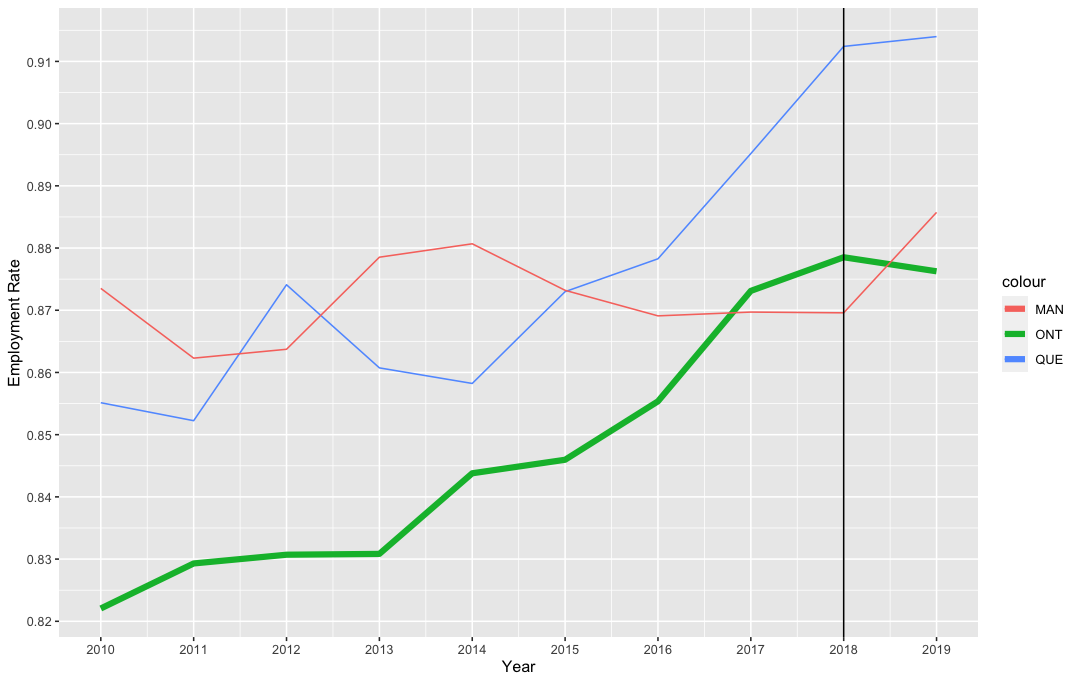
\includegraphics[scale=0.29]{employment_yearly}
		\end{center}
		We can see a parallel trend for QUE and ONT, but not for MAN and ONT. Let's have a look on the monthly employment rate:
		\begin{center}
			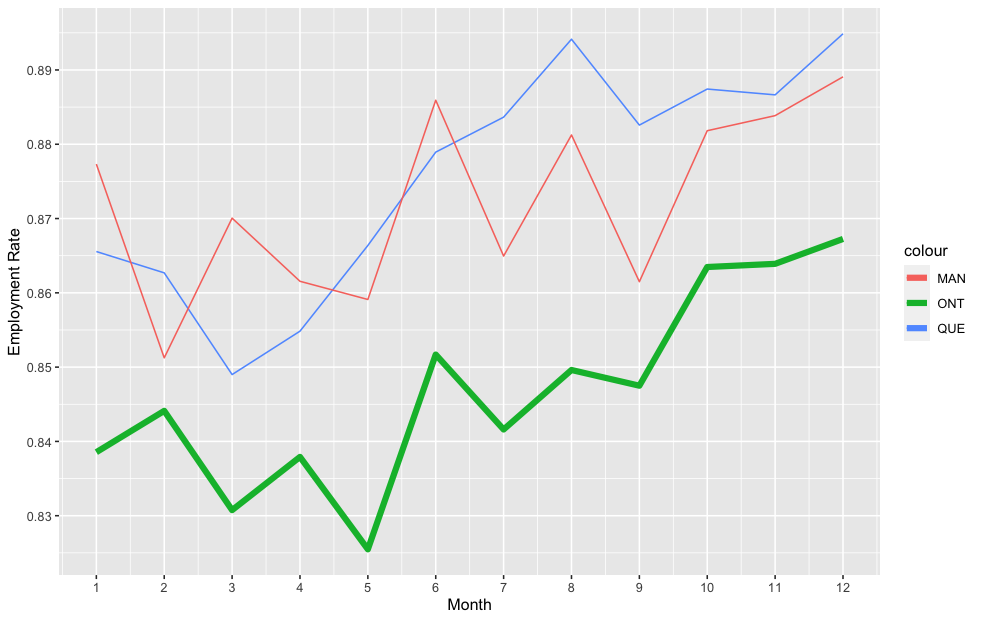
\includegraphics[scale=0.3]{employment_monthly}
		\end{center}
		There is some seasonality in the employment rate, during spring is less employment but it increases till the end of the year (maybe because employers need helping hands to handle the Christmas business?). We can see parallel trends between MAN and ONT after May and some weak parallel trends between QUE and ONT the whole year.
		\item Since I'll use the yearly data in the following tasks I use QUE as control group. Looking at some basic population statistics for states in Canada on Wikipedia QUE has more inhabitants than MAN and a similar population density as ONT. This means the employment rate is more stable during the years. \\
		After filtering the data and storing it in a data frame \texttt{df} we can specify the models (as usual look at the attached file for the whole R code):
		\begin{lstlisting}[tabsize=2]
# Model 1
m1 = lm(employed ~ D + T + D*T, data = df)

# Model 2
monthmatrix = matrix(0, nrow = nrow(df), ncol = 12)
for (i in 1:nrow(df)) {
	currentMonth = as.integer(df$month[i])
	monthmatrix[i, currentMonth] = 1
}
monthmatrix = monthmatrix[,-1] # base month = January
m2 = lm(employed ~ D + T + D*T + monthmatrix, data = df)
		\end{lstlisting}
		Before we come to the results let's think about good covariates. Good covariates correlate with the outcome variable but don't correlate with each other (no collinearity).
		\begin{lstlisting}[tabsize=2]
library(GGally)

# remove non-full columns
fullColumns = c()
for (colname in colnames(df)) {
	values = df[colname] %>% na.omit() %>% nrow()
	if (values == df[colname] %>% nrow()) {
	fullColumns = c(fullColumns, colname)
}
}
df = df[fullColumns]
ggcorr(df, label = TRUE)
		\end{lstlisting}
		Gives the following picture
		\begin{center}
			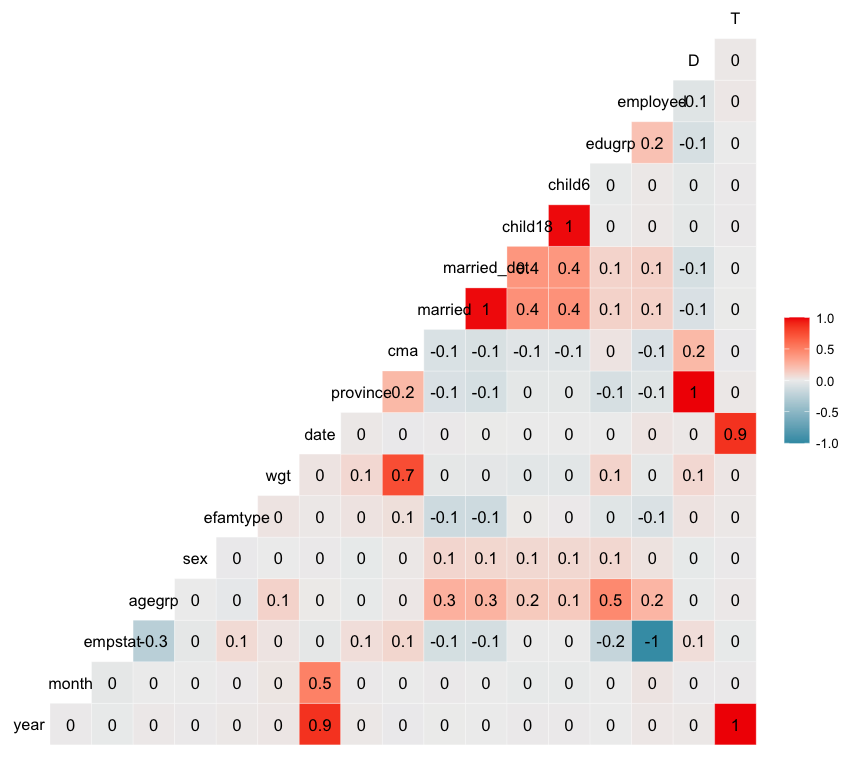
\includegraphics[scale=0.4]{corr}
		\end{center}
		If we look at the column with \texttt{employed} we can see that the following variables have a non-zero correlation with \texttt{employed}:
		\begin{itemize}
			\item \texttt{edugrp}: including in model 3
			\item \texttt{married}: including
			\item \texttt{married\_det}: not including because high correlation with \texttt{married}
			\item \texttt{cma}: not including because \texttt{cma} is the nearby Census Metropolitan Areas but it correlates with \texttt{province} which determines (= correlates with) \texttt{D}
			\item \texttt{province}: not including
			\item \texttt{efamtype}: including
			\item \texttt{agegrp}: including
			\item \texttt{empstat}: perfect correlation, not including, would lead to collinearity
		\end{itemize}
		This leads to the specification for model 3
		\begin{lstlisting}
m3 = lm(employed ~ D + T + D*T + monthmatrix + edugrp + married + efamtype + agegrp, data = df)
		\end{lstlisting}
		The results are
		% Table created by stargazer v.5.2.3 by Marek Hlavac, Social Policy Institute. E-mail: marek.hlavac at gmail.com
		% Date and time: So, Nov 13, 2022 - 12:12:14
		% Requires LaTeX packages: dcolumn 
		\begin{center}
			\begin{longtable}{lD{.}{.}{-3} D{.}{.}{-3} D{.}{.}{-3} } 
			\\ \hline 
			\hline \\ 
			 & \multicolumn{3}{c}{\textit{Dependent variable:}} \\ 
			\cline{2-4} 
			\\ & \multicolumn{3}{c}{employed} \\ 
			\\ & \multicolumn{1}{c}{(1)} & \multicolumn{1}{c}{(2)} & \multicolumn{1}{c}{(3)}\\ 
			\hline \\ 
			 D & -0.039^{***} & -0.039^{***} & -0.021^{***} \\ 
			  & (0.008) & (0.008) & (0.008) \\ 
			  & & & \\ 
			 T & 0.047^{***} & 0.046^{***} & 0.044^{***} \\ 
			  & (0.010) & (0.010) & (0.009) \\ 
			  & & & \\ 
			 monthmatrix1 &  & -0.031^{**} & -0.029^{**} \\ 
			  &  & (0.014) & (0.014) \\ 
			  & & & \\ 
			 monthmatrix2 &  & 0.010 & 0.009 \\ 
			  &  & (0.014) & (0.014) \\ 
			  & & & \\ 
			 monthmatrix3 &  & -0.014 & -0.016 \\ 
			  &  & (0.014) & (0.014) \\ 
			  & & & \\ 
			 monthmatrix4 &  & 0.042^{***} & 0.041^{***} \\ 
			  &  & (0.014) & (0.014) \\ 
			  & & & \\ 
			 monthmatrix5 &  & 0.104^{***} & 0.106^{***} \\ 
			  &  & (0.014) & (0.014) \\ 
			  & & & \\ 
			 monthmatrix6 &  & 0.142^{***} & 0.143^{***} \\ 
			  &  & (0.014) & (0.014) \\ 
			  & & & \\ 
			 monthmatrix7 &  & 0.101^{***} & 0.101^{***} \\ 
			  &  & (0.014) & (0.014) \\ 
			  & & & \\ 
			 monthmatrix8 &  & 0.015 & 0.015 \\ 
			  &  & (0.014) & (0.014) \\ 
			  & & & \\ 
			 monthmatrix9 &  & 0.030^{**} & 0.028^{**} \\ 
			  &  & (0.014) & (0.014) \\ 
			  & & & \\ 
			 monthmatrix10 &  & 0.022 & 0.019 \\ 
			  &  & (0.014) & (0.014) \\ 
			  & & & \\ 
			 monthmatrix11 &  & 0.018 & 0.023^{*} \\ 
			  &  & (0.014) & (0.014) \\ 
			  & & & \\ 
			 edugrp &  &  & 0.073^{***} \\ 
			  &  &  & (0.005) \\ 
			  & & & \\ 
			 married &  &  & 0.073^{***} \\ 
			  &  &  & (0.010) \\ 
			  & & & \\ 
			 efamtype &  &  & -0.006^{***} \\ 
			  &  &  & (0.001) \\ 
			  & & & \\ 
			 agegrp &  &  & 0.192^{***} \\ 
			  &  &  & (0.007) \\ 
			  & & & \\ 
			 D:T & -0.046^{***} & -0.046^{***} & -0.045^{***} \\ 
			  & (0.012) & (0.012) & (0.012) \\ 
			  & & & \\ 
			 Constant & 0.586^{***} & 0.551^{***} & 0.177^{***} \\ 
			  & (0.007) & (0.012) & (0.015) \\ 
			  & & & \\
			\hline 
			Observations & \multicolumn{1}{c}{28,647} & \multicolumn{1}{c}{28,647} & \multicolumn{1}{c}{28,647} \\ 
			R$^{2}$ & \multicolumn{1}{c}{0.004} & \multicolumn{1}{c}{0.014} & \multicolumn{1}{c}{0.089} \\ 
			Adjusted R$^{2}$ & \multicolumn{1}{c}{0.004} & \multicolumn{1}{c}{0.014} & \multicolumn{1}{c}{0.089} \\ 
			Residual Std. Error & \multicolumn{1}{c}{0.494} & \multicolumn{1}{c}{0.492} & \multicolumn{1}{c}{0.473} \\ 
			F Statistic & \multicolumn{1}{c}{41.232$^{***}$} & \multicolumn{1}{c}{30.059$^{***}$} & \multicolumn{1}{c}{156.306$^{***}$} \\ 
			\hline 
			\textit{Note:}  & \multicolumn{3}{r}{$^{*}$p$<$0.1; $^{**}$p$<$0.05; $^{***}$p$<$0.01} \\ 
			\end{longtable} 
		\end{center}
		We see that the treatment effect (coefficient for \texttt{D:T}) is significant, negative and nearly the same in all three models. The added covariates in model 3 increase the $R^2$ (although it is still extremely low) and we can see the seasonality effects in summer (\texttt{monthmatrix4} is for May etc.).
		\item Specification for model 4:
		\begin{lstlisting}[tabsize=2]
timematrix = matrix(0, nrow = nrow(df), ncol = 6)
colnames(timematrix) = c("2014", "2015", "2016", "2017", "2018", "2019")
for (i in 1:nrow(df)) {
	currentYear = as.integer(df$year[i])
	timematrix[i, currentYear - 2014 + 1] = 1
}
timematrix = timematrix[,-4] # base year = 2017
monthmatrix = matrix(0, nrow = nrow(df), ncol = 12)
for (i in 1:nrow(df)) {
	currentMonth = as.integer(df$month[i])
	monthmatrix[i, currentMonth] = 1
}
monthmatrix = monthmatrix[,-1] # base month = January
m4 = lm(employed ~ D + timematrix + monthmatrix + timematrix*D, data = df)
		\end{lstlisting}
		We can collect the estimates and standard errors with \texttt{coef(m4)} and \texttt{coef(summary(m4))}. The the 95\%-CI is (assuming a normal distribution because we have lots of observations $\Rightarrow$ high degrees of freedom for $t$-distribution)
		\begin{align}
			CI = \hat{\beta} + z_{0.975}\cdot SE(\hat{\beta}) \notag
		\end{align}
		Plotting these gives us
		\begin{center}
			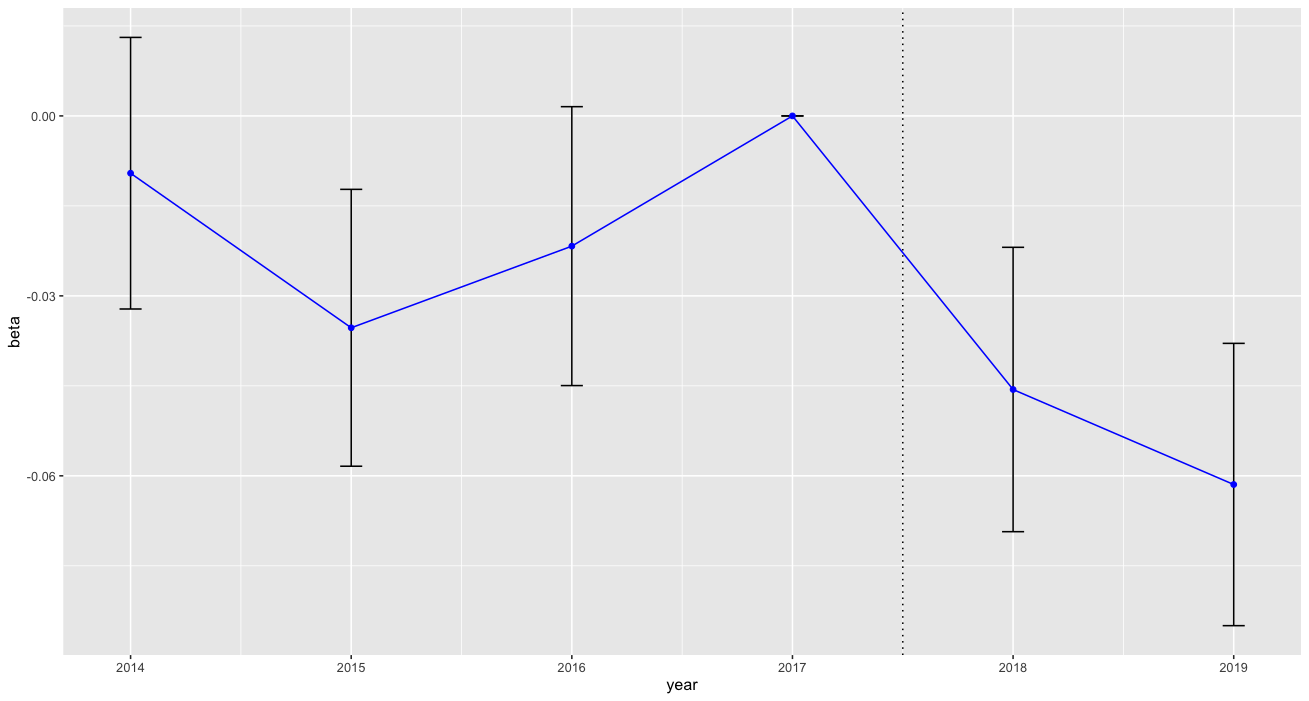
\includegraphics[scale=0.3]{estimators}
		\end{center}
		For our parallel trends assumption we want $\hat{\beta}_{2014} = \hat{\beta}_{2015} = \hat{\beta}_{2016} = 0$ which we can get for 2014 and 2016 but not for 2015. We can rule out pre-emptive behaviour because 2015 no one could have known of this policy (maybe some members of government). At least 2018 and 2019 we have clear negative treatment effects.
		\item We need to make the additional assumption that we have parallel trends on monthly trends.
		\item The best approach would be to do whole section again but this time averaging employment rate not on a yearly basis but on a monthly basis giving us coefficients $\beta_{2014,Jan}$, $\beta_{2014,Feb}$, ..., $\beta_{2019,Dez}$ and then testing for $\beta_{2017,Jun} = ... = \beta_{2017,Dec} = 0$. I'll go another approach by just plotting the employment rate of the year 2017. If there is pre-emptive behaviour we should see it:
		\begin{lstlisting}[tabsize=2]
employmentRateMonthly2017 = data.frame(cbind(1:12, rep(0, 12), rep(0, 12)))
colnames(employmentRateMonthly2017) = c("Month", "QUE", "ONT")
for (prov in 5:6) {
	empRateForMonth = c()
	for (m in 1:12) {
		employed = data %>% filter(province == prov) %>% filter(month == m) %>% filter(year == 2017) %>% filter(between(agegrp, 1, 2)) %>% filter(between(empstat, 1, 2)) %>% nrow()
		population = data %>% filter(province == prov) %>% filter(month == m) %>% filter(year == 2017) %>% filter(between(agegrp, 1, 2)) %>% filter(between(empstat, 1, 3)) %>% nrow()
		empRateForMonth = c(empRateForMonth, employed/population)
	}
	if (prov == 5) employmentRateMonthly2017$QUE = empRateForMonth
	if (prov == 6) employmentRateMonthly2017$ONT = empRateForMonth
}
ggplot(employmentRateMonthly2017, aes(x = Month)) + 
	geom_line(aes(y = QUE, color = "QUE")) +
	geom_line(aes(y = ONT, color = "ONT"), size = 2) +
	ylab("Employment Rate") + 
	xlab("Month of 2017") + 
	scale_x_continuous(breaks = seq(1, 12, by = 1)) +
	scale_y_continuous(breaks = seq(0.1, 1, by = 0.01)) + 
	geom_vline(xintercept = 6)
		\end{lstlisting}
		gives us
		\begin{center}
			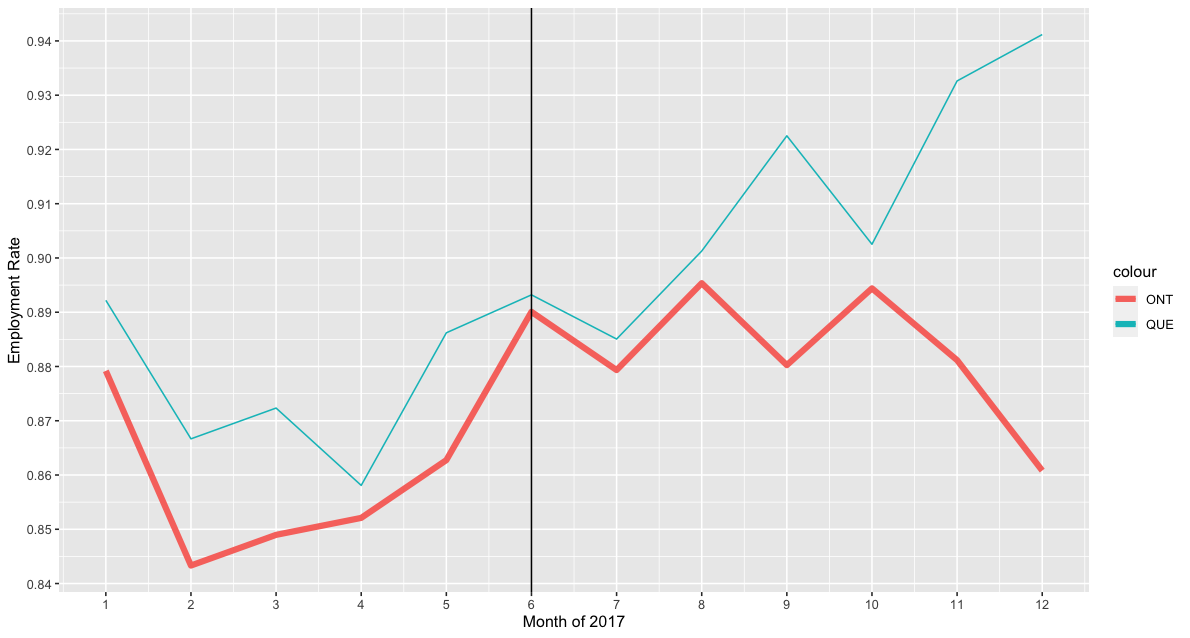
\includegraphics[scale=0.3]{preemptive}
		\end{center}
		The trends look pretty much the same but they differ when it comes to the end of the year. Instead of going up as seen in (b) for Christmas business the employment rate in ONT goes down. Maybe this is has nothing to do with the upcoming policy and Christmas business isn't booming as usual but it can also be pre-emptive behaviour.
		\item There might be bigger changes in the labour market in ONT than just the minimum wage raise. If there is than older people (older people have most likely worked for many years and therefore earn more than minimum wage) would be affected to. We can test this by looking only at ONT and using as control group people older than 24. We could go one step further and not use age as a separator but \texttt{HRLYEARN} and investigate what's happening to the employment rate of low-earners vs. high-earners. Problem here is that 25\% of our dataset has no information of \texttt{HRLYEARN} (see plot of missing values at the start of this task).
		\item Literature suggests that $\beta_{2018} = \beta_{2019} = 0$ which is not the case for my estimators, the 95\%-CI doesn't include 0. Since I only look at data from ONT maybe other Ontario-specific effects have influenced my result and we should use more data from other parts of the world too. \\
		Interestingly after playing around with the data I found an interesting R command: \texttt{step()} which does a backward model selection. I start with every covariate included (and excluding covariates with perfect collinearity) and step by step covariates get removed to make the AIC smaller:
		\begin{lstlisting}
step(lm(employed ~ . -year - date - province + D:T, data = df))
		\end{lstlisting}
		leads to the following model:
		\begin{lstlisting}
lm(formula = employed ~ month + empstat + agegrp + sex + efamtype + cma + married + married_det + child6 + D + T, data = df)
		\end{lstlisting}
		which doesn't include the treatment effect \texttt{D:T}. With other words: The employment status can't be enough explained by minimum wage raise or $\beta = 0$.
	\end{enumerate}

	\section*{Section E: Synthetic Control}
	\textit{I used R for this task. The code I've written is attached but for comparison I asked a friend of mine to run the provided STATA commands. We got different results and - as mentioned in the forum - no one knows why. I think it might be the different optimisation algorithm. But in this task I will reference to the results R gave to me.}
	
	After fitting the models I got
	\begin{center}
		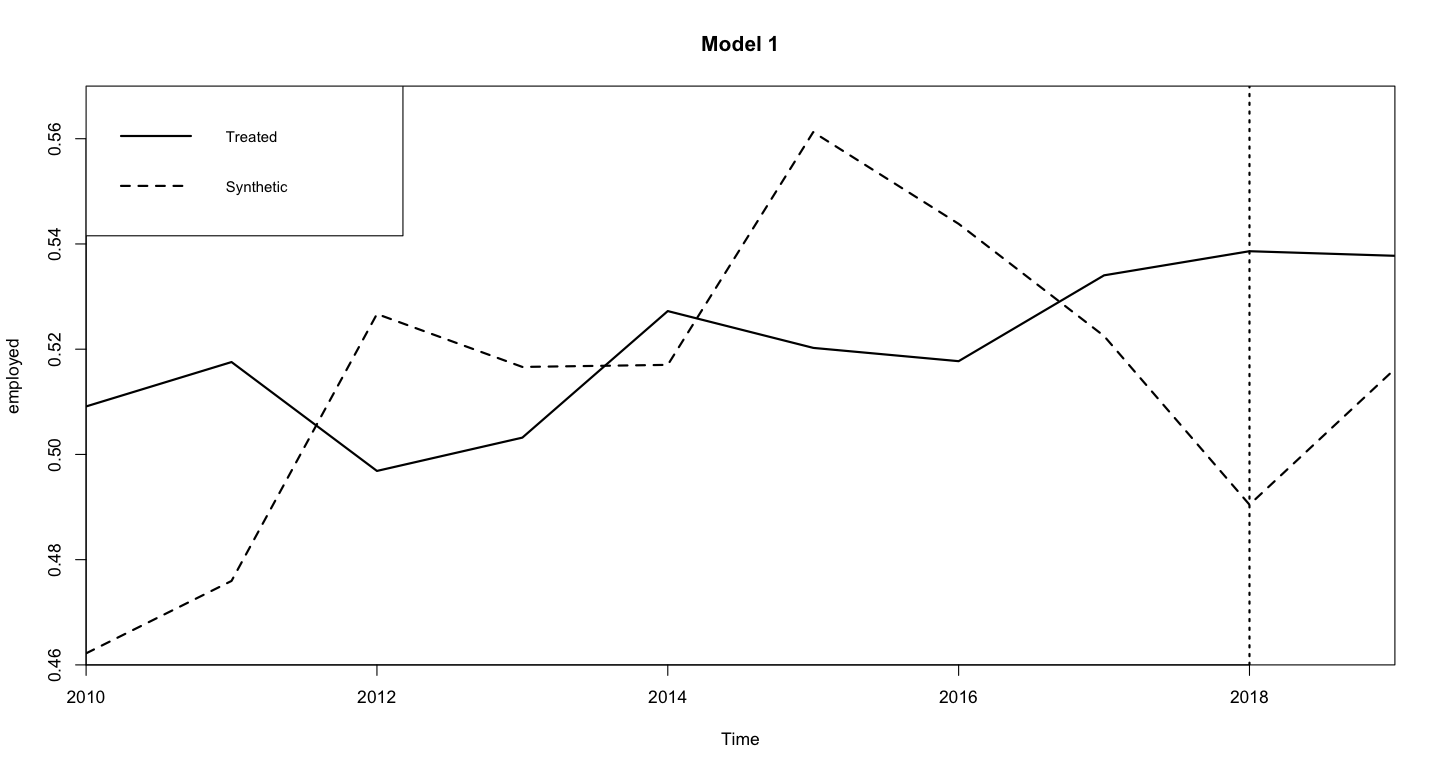
\includegraphics[scale = 0.15]{model1}
		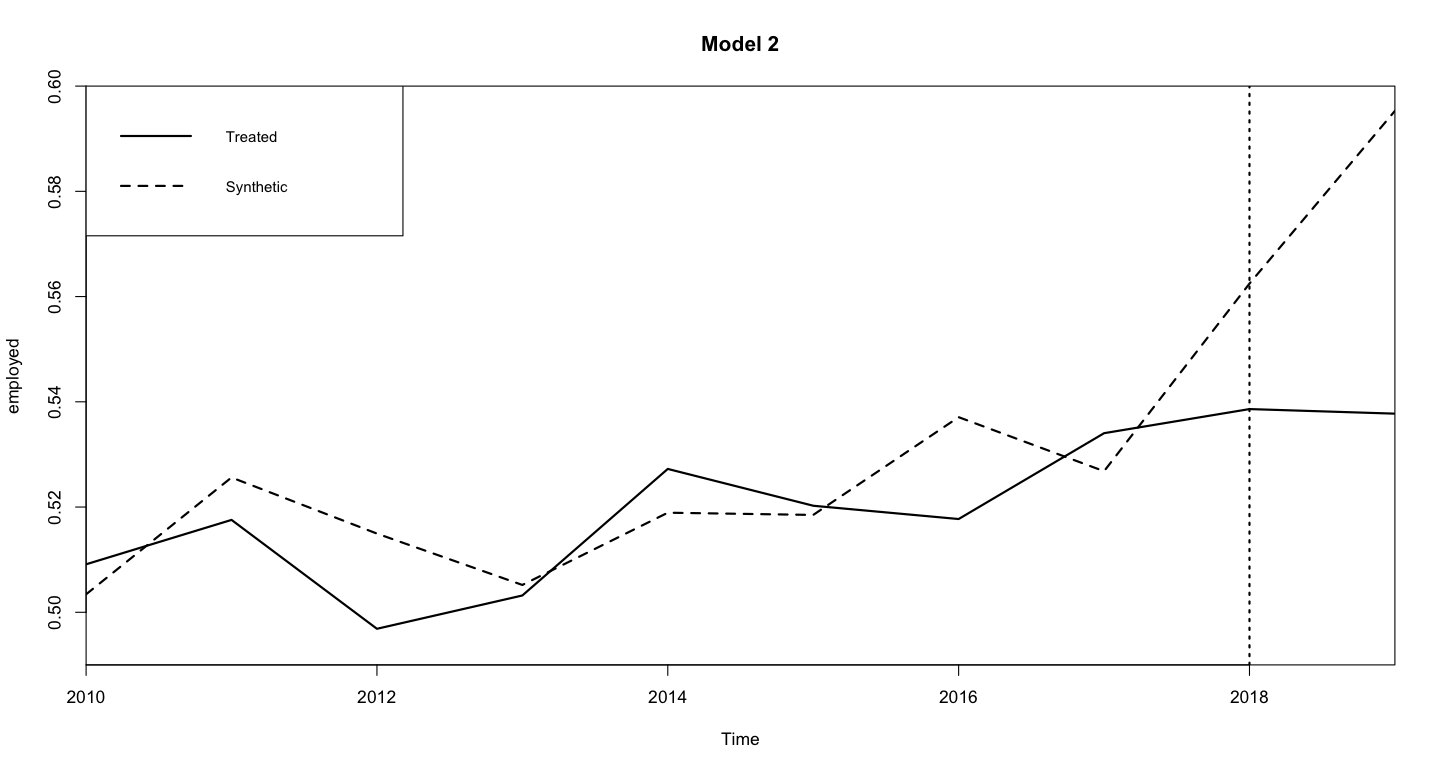
\includegraphics[scale = 0.15]{model2}
		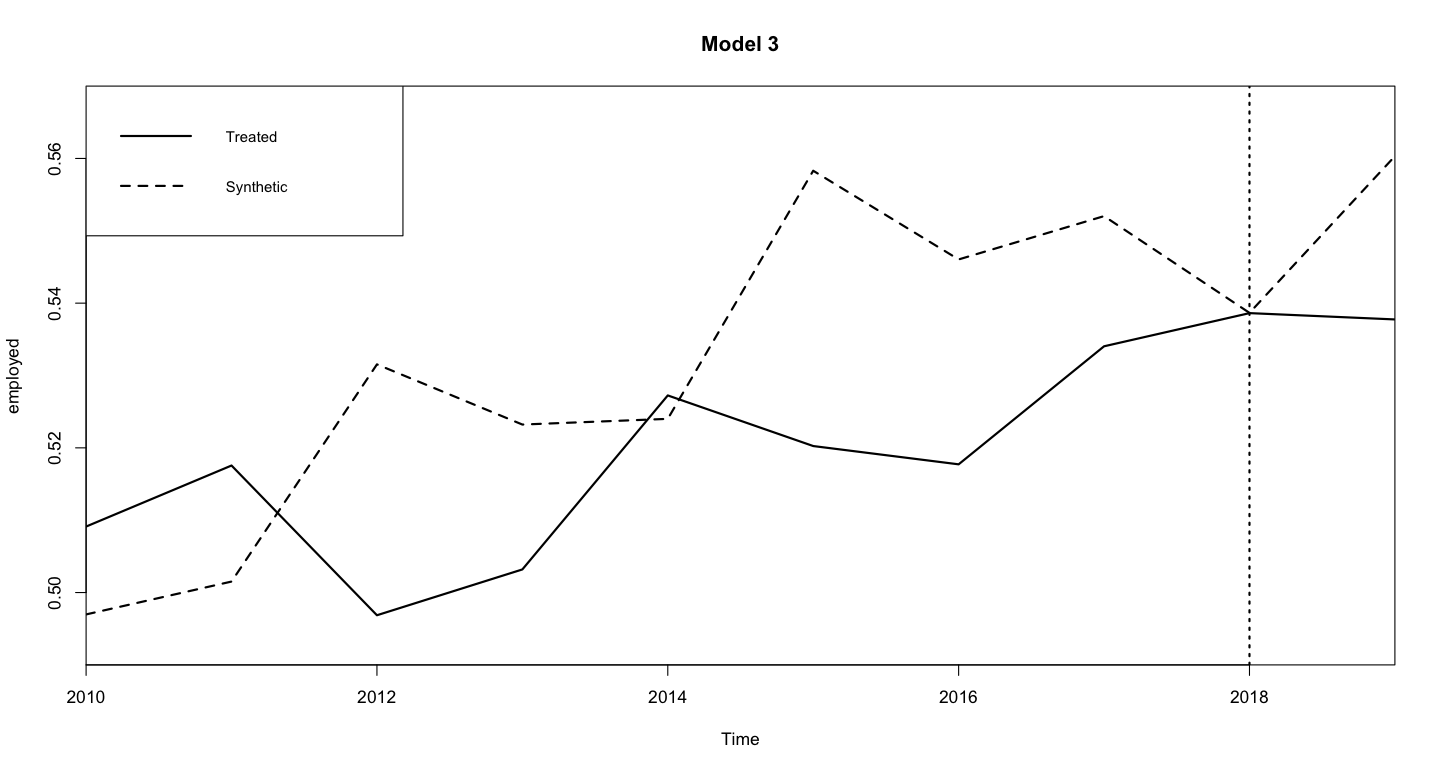
\includegraphics[scale = 0.15]{model3}
		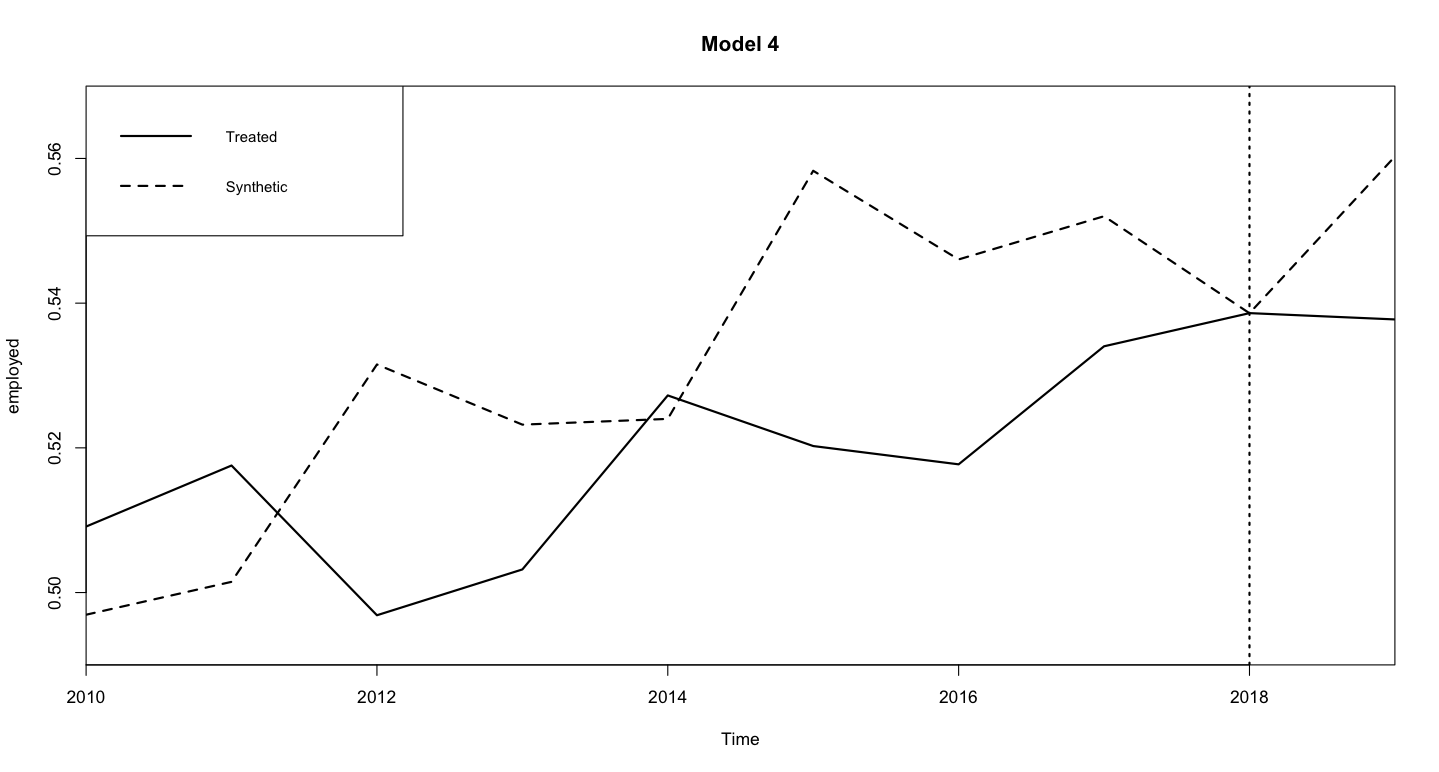
\includegraphics[scale = 0.15]{model4}
	\end{center}
	Model 1 and 2 got the same weights as in STATA but a parallel trend can't be seen. Model 2 has a better fit in the pre-treatment period but in post-treatment it is way off. Model 3 and 4 look in the graph the same but the weights have a minimal difference. STATA will give different weights in model 3 and 4.
	
	The weights are
	\begin{center}
		\begin{tabular}{c|c|c|c|c}
			\textbf{Province} & \textbf{Model 1} & \textbf{Model 2} & \textbf{Model 3} & \textbf{Model 4} \\
			\hline
			 NFL & 0.73710714 & $1.935781\cdot 10^{-4}$ & 0.4018604 & 0.4022425 \\			
			 PEI & 0.02294339 & $3.662704\cdot 10^{-5}$ & $1.412148\cdot 10^{-5}$ & $6.811447\cdot 10^{-7}$ \\
			 NS & 0.04418981 & $1.263440\cdot 10^{-4}$ & 0.3229095 & 0.3225237 \\
			 NB & 0.08904221 & $0.9994246$ & $1.072118\cdot 10^{-6}$ & $4.512253\cdot 10^{-8}$ \\
			 QUE & 0.02098721 & $3.396839\cdot 10^{-5}$ & $2.711164\cdot 10^{-9}$ & $3.944902\cdot 10^{-8}$ \\
			 MAN & 0.01914771 & $4.130334\cdot 10^{-5}$ & $1.443463\cdot 10^{-6}$ & $8.024621\cdot 10^{-8}$ \\
			 SASK & 0.01552675 & $3.204996\cdot 10^{-5}$ & $8.581286\cdot 10^{-7}$ & $6.041839\cdot 10^{-8}$ \\
			 ALB & 0.01555429 & $3.296223\cdot 10^{-5}$ & $4.928783\cdot 10^{-6}$ & $5.619475\cdot 10^{-7}$ \\
			 BC & 0.03550150 & $7.858791\cdot 10^{-5}$ & 0.2752076 & 0.2752323 \\
		\end{tabular}
	\end{center}
	For better readability I created a graph for the weights
	\begin{center}
		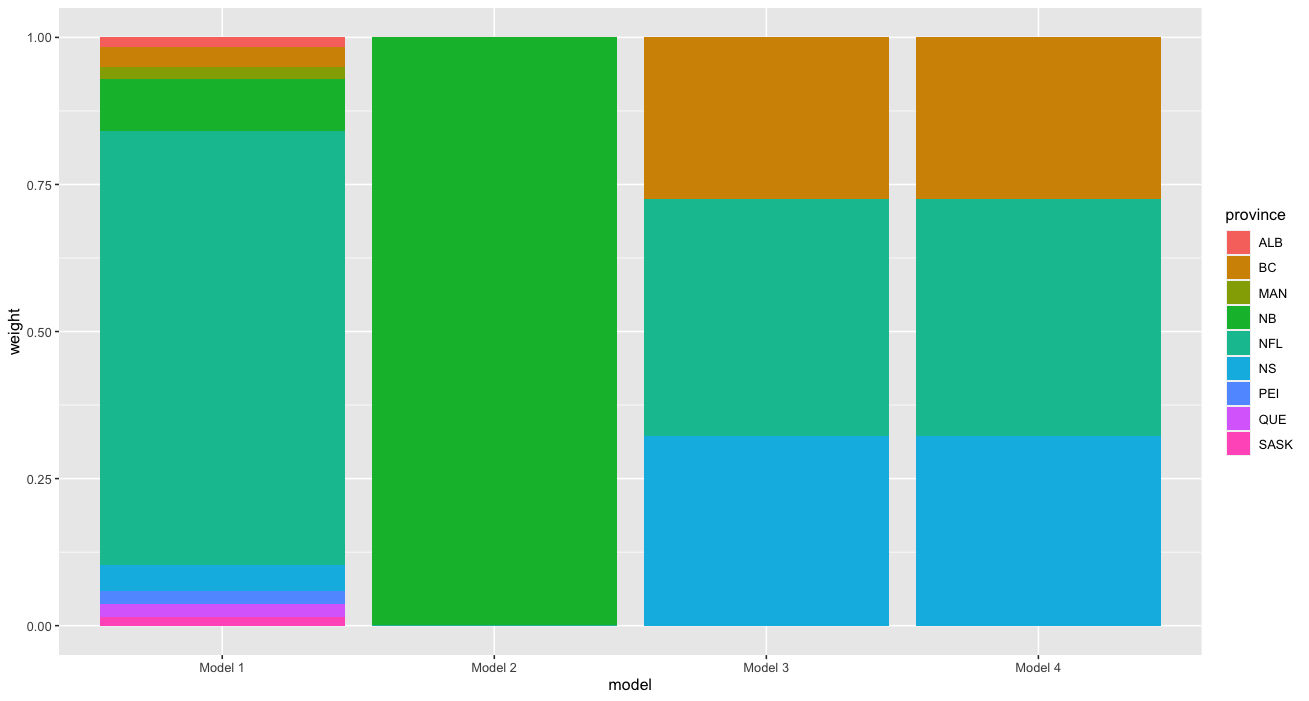
\includegraphics[scale=0.35]{weights}
	\end{center}
	According to Model 2 the province NB (New Brunswick) is a control group for Ontario. New Brunswick has 2.09\% of Canada's population while Ontario has 38.45\%; population density is 10.9 for NB and 15.2 per km$^2$ for ONT. But in general I don't think that NB is a good control group, they are not similar. The other models build their synthetic control group by a large weight from NFL (Newfoundland and Labrador) which has even less inhabitants than NB (1.38\%) and a population density of 1.4 per km$^2$. Model 3 and 4 include in their synthetic control group BC (British Columbia) which is the third-largest province (13.52\% of population) and has a nearly identical market income per capita than ONT (36,723 CAD vs. 36,298 CAD). The third part of the synthetic control group of model 3 and 4 is NS (New Scotia) which has only 2.62\% of population but a population density of 18.4 per km$^2$. The market income per capita for NS is around 30,000 CAD.\footnote{data from \url{https://en.wikipedia.org/wiki/Population_of_Canada_by_province_and_territory} and \url{https://en.wikipedia.org/wiki/List_of_Canadian_provinces_and_territories_by_gross_domestic_product}}
	
	From my point of view are model 1 and 2 not suitable as control group for Ontario. Model 3 and 4 are better but the graphs with the predicted employment rate don't convince me. Especially since the paper \cite{Abadie2015} looks much more promising in it's plots and predictions.
	
	\printbibliography 

\end{document}